\subsubsection{Ý tưởng}

Counting Sort là một thuật toán sắp xếp dựa trên phép đếm số lần xuất hiện của các phần tử trong mảng. Thuật toán này chỉ hoạt động với các mảng có giá trị không âm và có giới hạn về giá trị của các phần tử trong mảng. \cite{cormen2001}

\subsubsection{Mã giả}

\begin{algorithm}[H]
\caption{Counting Sort}
\begin{algorithmic}[1]
\Function{CountingSort}{$arr, n$}
    \State $max \gets \text{max}(arr)$
    \State $count \gets [0] * (max + 1)$
    \State $output \gets [0] * n$
    \For{$i \gets 0$ \textbf{to} $n - 1$}
        \State $count[arr[i]] \gets count[arr[i]] + 1$
    \EndFor
    \For{$i \gets 1$ \textbf{to} $max$}
        \State $count[i] \gets count[i] + count[i - 1]$
    \EndFor
    \For{$i \gets n - 1$ \textbf{downto} $0$}
        \State $output[count[arr[i]] - 1] \gets arr[i]$
        \State $count[arr[i]] \gets count[arr[i]] - 1$
    \EndFor
    \State \textbf{return} $output$
\EndFunction
\end{algorithmic}
\end{algorithm}

\subsubsection{Ví dụ}

Giả sử ta có mảng $arr = [42, 17, 93, 58, 21, 76, 34]$ và ta muốn sắp xếp mảng này bằng thuật toán Counting Sort.
\begin{enumerate}
    \item \textbf{Bước 1}: Tính số lần xuất hiện của các phần tử trong mảng $arr$ và lưu vào mảng $count$.\\Mảng $count$ trong hình được lược bỏ các phần tử có giá trị bằng $0$.
    \item \textbf{Bước 2}: Tính số lần xuất hiện của các phần tử nhỏ hơn hoặc bằng phần tử hiện tại trong mảng $count$.
    \item \textbf{Bước 3}: Sắp xếp mảng $arr$ vào mảng $output$ dựa trên số lần xuất hiện của các phần tử trong mảng $count$.
\end{enumerate}

\begin{figure}[H]
    \centering
    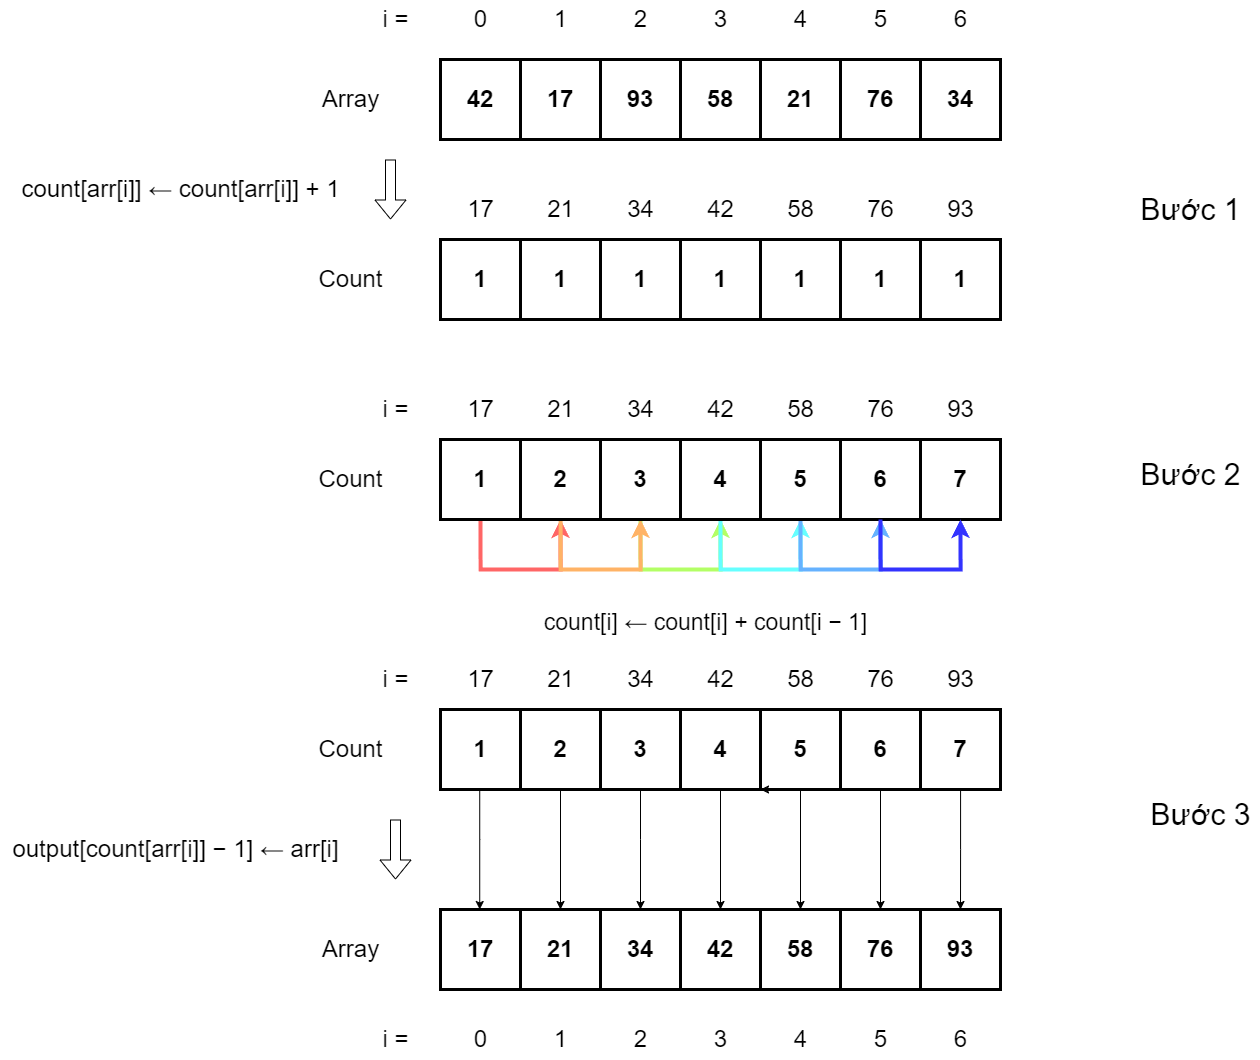
\includegraphics[width=0.75\linewidth]{img/counting_sort/1.png}
    \caption{Quá trình thực hiện Counting Sort}
\end{figure}

\subsubsection{Độ phức tạp}

\begin{itemize}
    \item Độ phức tạp thời gian: $\mathcal{O}(n + k)$
    \item Độ phức tạp không gian: $\mathcal{O}(n + k)$
    \item Ưu điểm:
        \begin{itemize}
            \item Độ phức tạp thời gian tốt nhất trong các thuật toán sắp xếp: $\mathcal{O}(n)$
            \item Không sử dụng so sánh giữa các phần tử
        \end{itemize}
    \item Nhược điểm:
        \begin{itemize}
            \item Chỉ hoạt động với các mảng có giá trị không âm và có giới hạn về giá trị của các phần tử
            \item Không thể sắp xếp các mảng có số thập phân
        \end{itemize}
    \item Tính ổn định: \textit{Counting Sort} là một thuật toán ổn định. Điều này có nghĩa là nếu có hai phần tử bằng nhau, thì chúng sẽ không bị đảo lộn thứ tự sau khi sắp xếp.
    \item Ứng dụng:
        \begin{itemize}
            \item Sắp xếp các mảng có giá trị không âm và có giới hạn về giá trị của các phần tử
        \end{itemize}
\end{itemize}
